\documentclass{beamer}
\usepackage[english]{babel}
\usepackage[latin1]{inputenc}
\usepackage[T1]{fontenc}
\usepackage{amssymb}
\usepackage{amsmath}
\usepackage{booktabs}
\usepackage{verbatim}
\usepackage{caption}
\usepackage{float}
%\usepackage{natbib}
\usepackage{csquotes}
\usepackage{sansmathaccent}
\usepackage{subfigure}
\usepackage{multicol}
\pdfmapfile{+sansmathaccent.map}
\usepackage{mathtools}
\def \ourFigPath {../../} 
\def \MainFigures{../Draft_Summer2018/MainFigures}
\def \ourTablePath {../../Tables/} 
\def\myFigWidth{2.0in}


\setbeamersize{text margin left=5mm,text margin right=12mm} 
%
\font\reali=msbm10 at 12pt
% subsets of real numbers
\newcommand{\numberset}{\mathbb}
\newcommand{\real}{\hbox{\reali R}}
\newcommand{\N}{\numberset{N}}
\newcommand{\realp}{\hbox{\reali R}_{\scriptscriptstyle +}}
\newcommand{\realpp}{\hbox{\reali R}_{\scriptscriptstyle ++}}
\newcommand{\virgolette}[1]{``#1''}
%

\author[Brianti, G\'ati]{Marco Brianti and Laura G\'ati}

\institute[Boston College]{Boston College}


\title[ICT]{ICT and Future Productivity: Evidence and Theory of a GPT}

\date{June 2018}

\usetheme{Warsaw}


\begin{document}


\begin{frame}

\maketitle


\end{frame}


% Structure:
% 1. Motivation: the triumvirate of medium-run BC, ICT and SVAR literature on things that affect future stuff
% 2. This paper: 1. run a VAR with ICT identified properly, get surprising results  2. Try to interpret those along the ICT literature: is ICT a GPT?
% 3. Show VAR
% 4. Show model



%%%%%%% Slide %%%%%%
\begin{frame}
	\frametitle{Motivation}
	
	\begin{itemize}
		
		\item Point of departure: medium-run business cycle models \`a la Comin \& Gertler (2006).
		
		\
		
		\item Key prediction: BC fluctuations of a particular kind of investment (research \& development (R\&D) $\rightarrow$ adoption) lead total factor productivity (TFP)
		
		\
		
	\item The Great Recession 2008 casts doubt on whether this is all of the story (Fernald et al. (2017)).
	
	\
	
	
	\end{itemize} 

\end{frame}
%%%%%%%%%%%%%%%%%

%%%%%%% Slide %%%%%%
\begin{frame}
	\frametitle{Wrong timing}
	
		\vspace{-1cm}
	\noindent
	\begin{figure}
		\centering
		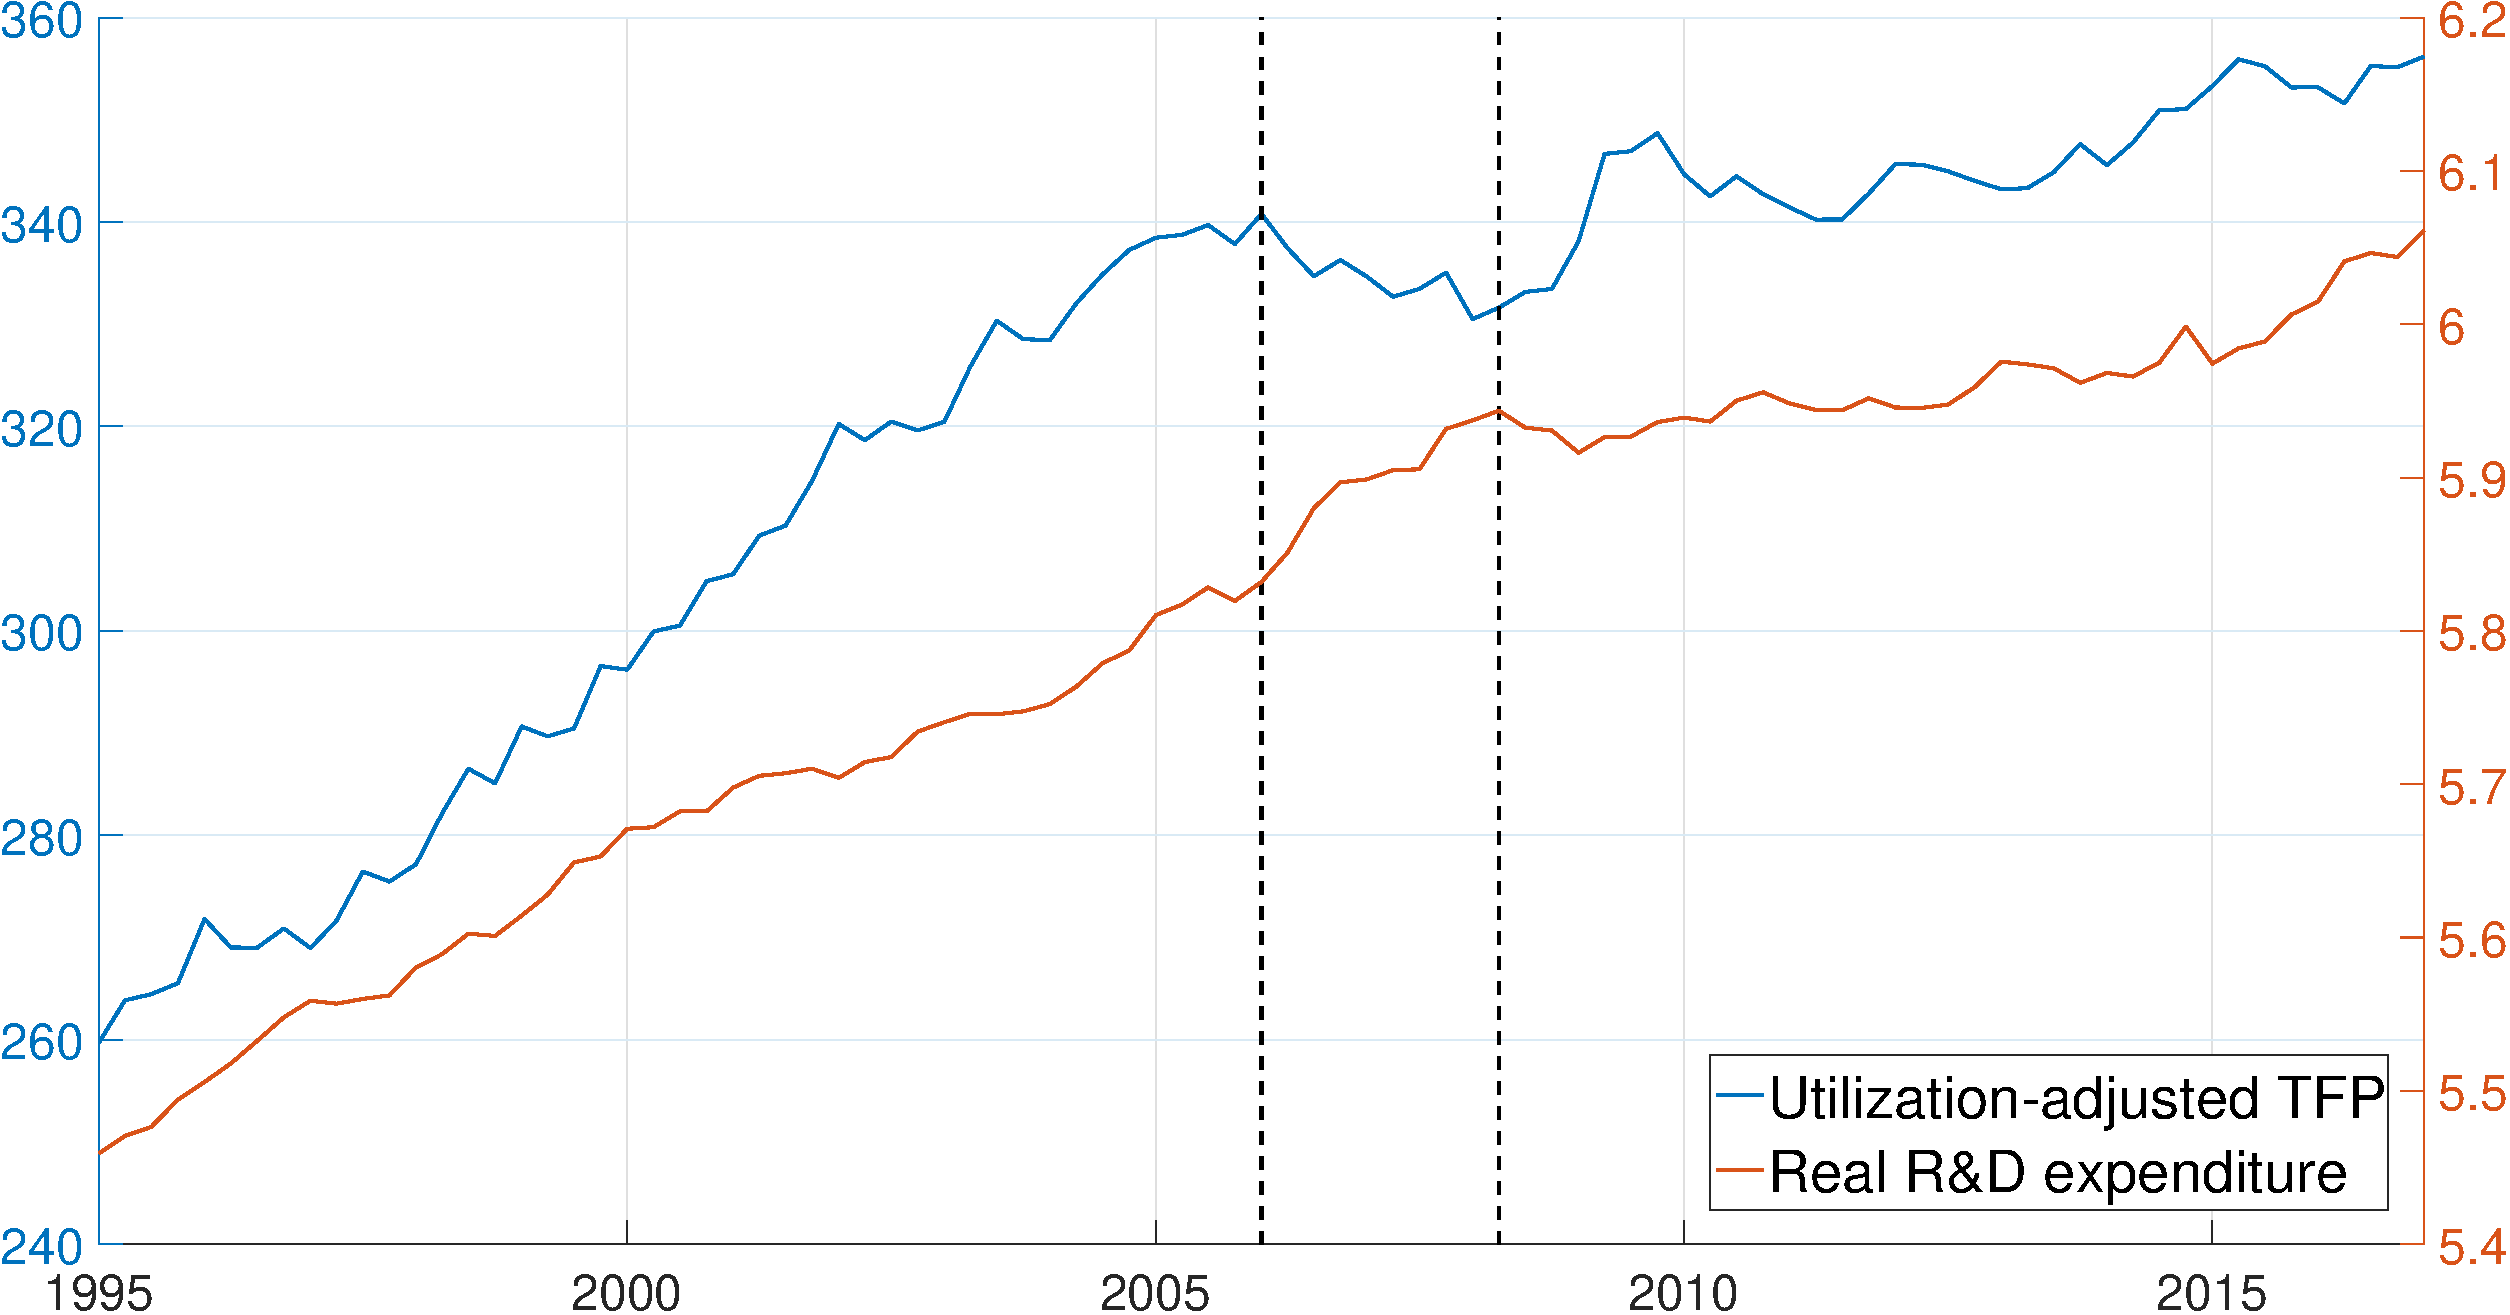
\includegraphics[scale=0.28]{\ourFigPath Figures/fig_RD_level_macrolunch_30-Nov-2017_11_31_04}
	\end{figure}
	
	Fernald et al. (2017): ``R\&D and adoption cannot be the whole story''.

\end{frame}
%%%%%%%%%%%%%%%%%


%%%%%%% Slide %%%%%%
\begin{frame}
	\frametitle{}
	
		\noindent
	\begin{figure}
		\centering
		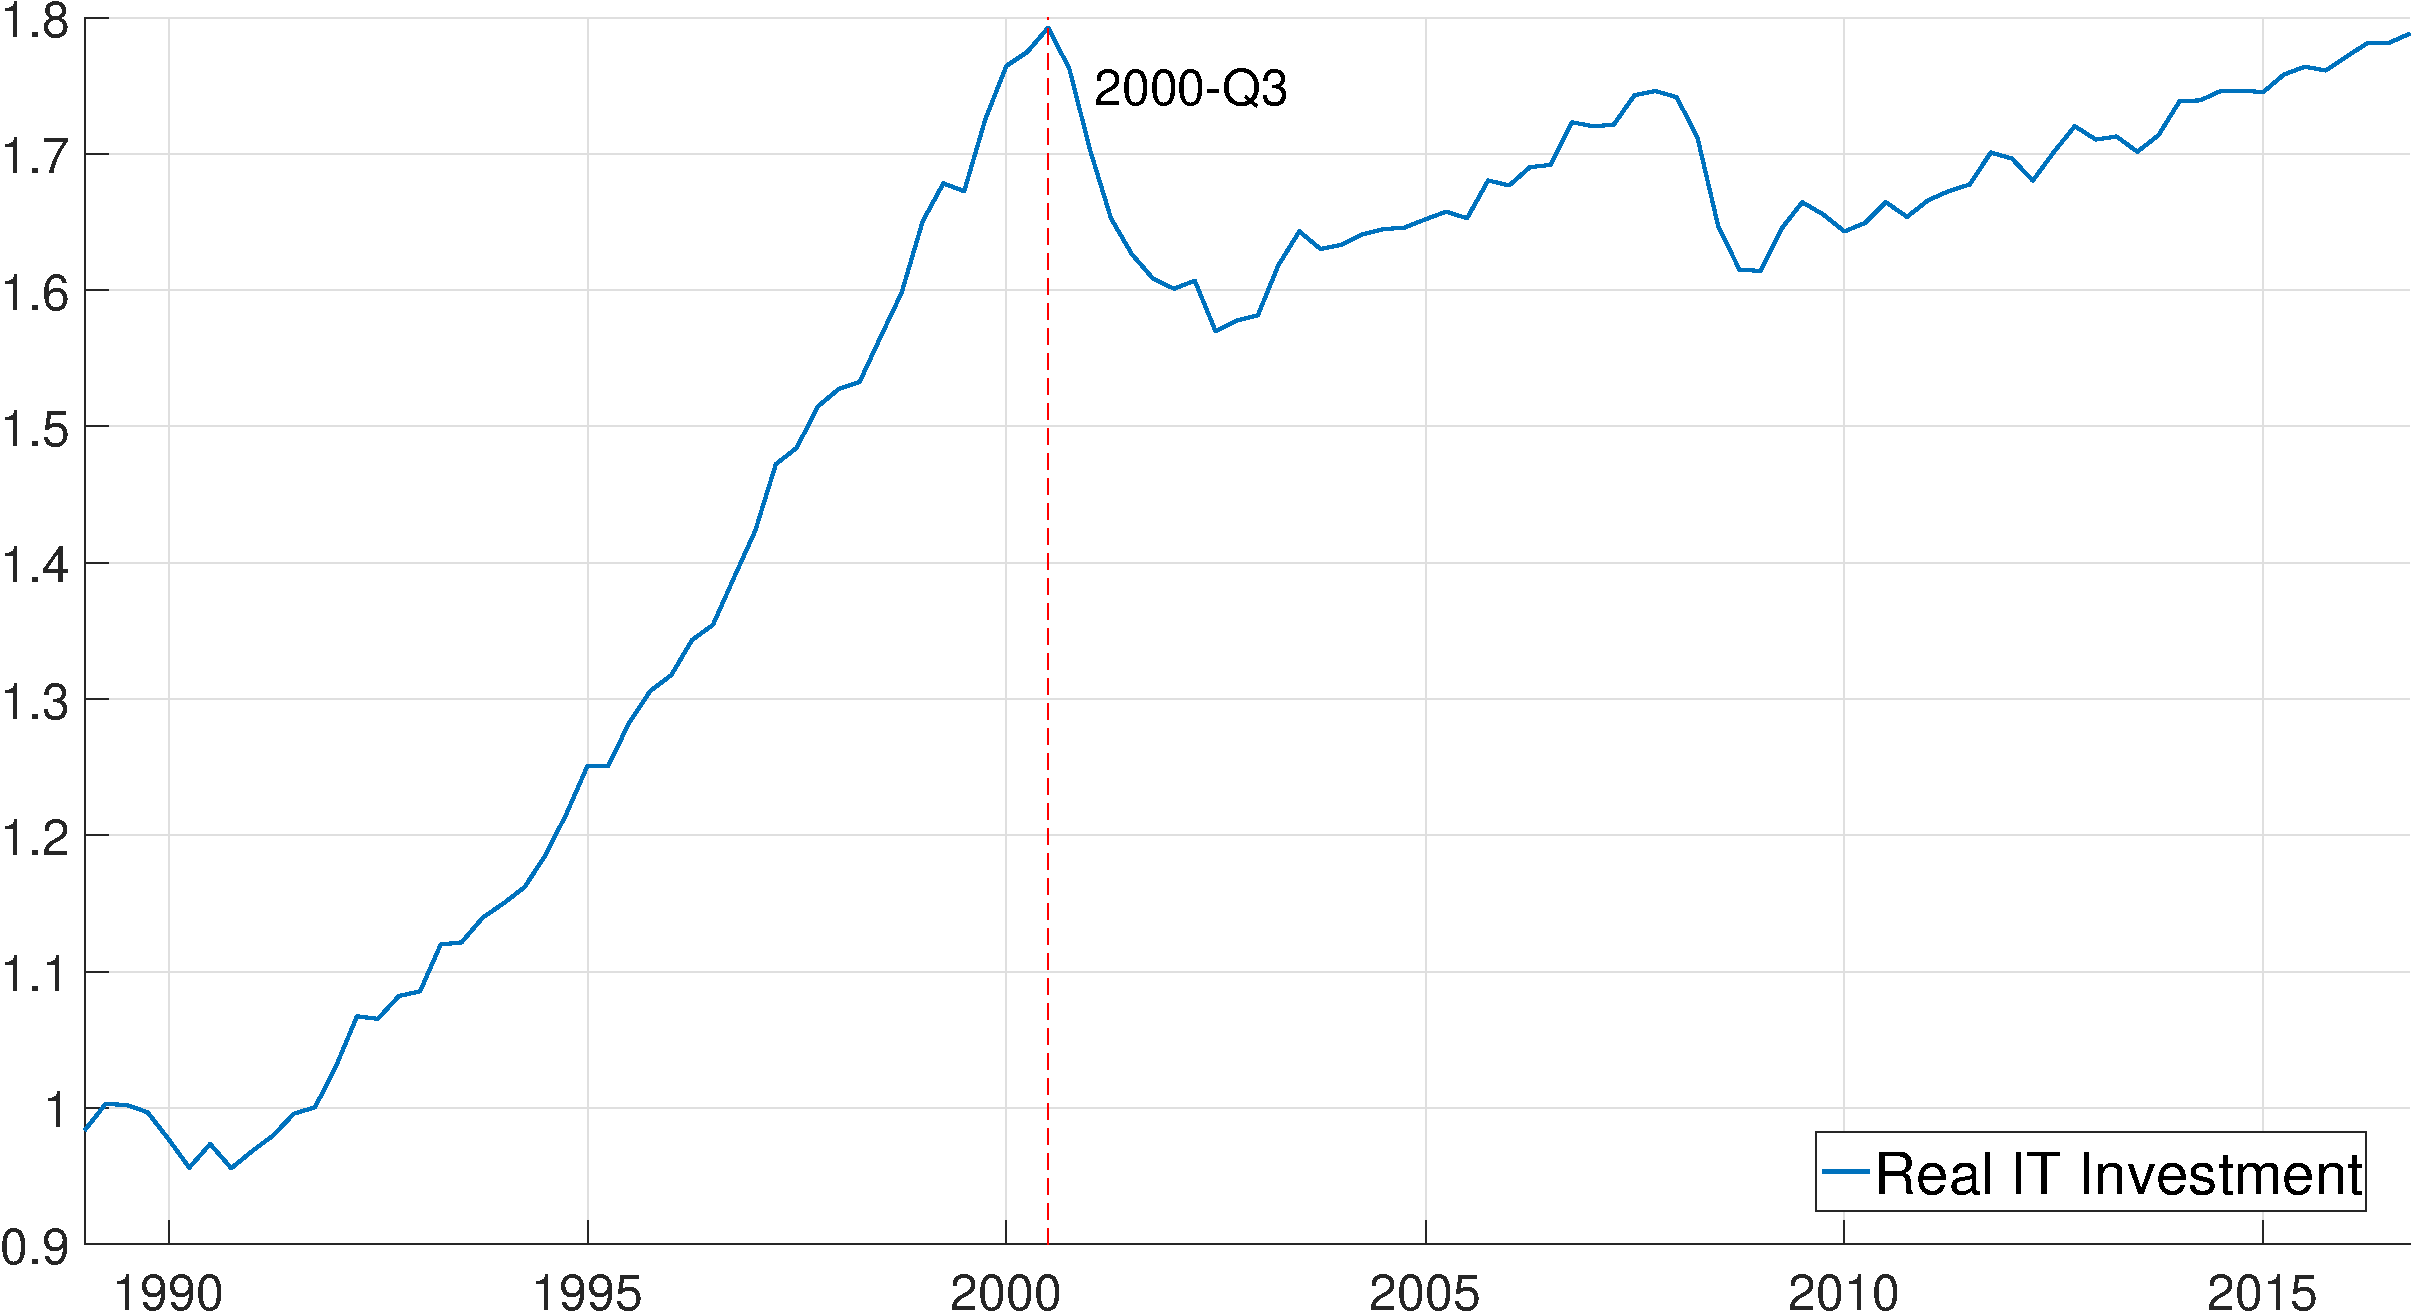
\includegraphics[scale=0.29]{\ourFigPath Figures/fig_IT_level_macrolunch_30-Nov-2017_11_37_26}
	\end{figure}
	
	\begin{itemize}
		
		\item [$\rightarrow$] A variable with at least the right timing is investment in information and communication technologies (ICT)
	
	
	\end{itemize} 

\end{frame}
%%%%%%%%%%%%%%%%%


%%%%%%% Slide %%%%%%
\begin{frame}
	\frametitle{This paper}
	
	\begin{enumerate}
	\item Stick ICT investment (ICT-I) in a VAR and explore how an identified shock to this affects TFP.
	\item [] ICT shock = a shock to the productivity of the ICT sector today
	
	\
	
	\begin{itemize}
	\item [$\rightarrow$] A shock to ICT leads to substantial TFP increases over the medium-run.
	\end{itemize}

\
	
    \item Draw on the conclusions of the ICT literature (references!) to build a structural model to interpret the results. 
    
    \
    
    	\begin{itemize}
	\item [$\rightarrow$] ICT literature: ICT is a general-purpose technology (GPT).
	
	\
	
	\item[$\Rightarrow$] Estimate a two-sector endogenous growth model to ask whether aggregate data supports this interpretation. 
	\end{itemize}
	
	\end{enumerate} 

\end{frame}
%%%%%%%%%%%%%%%%%


%%%%%%%%%%%%%%%%%%%%%%%%%%%%%%%% HERE HERE HERE
% - complete ICT literature references 
% - implement roadmap
% - edit title

%%%%%%% Slide %%%%%%
\begin{frame}
	\frametitle{Related literature}
	
	\begin{enumerate}
	\item Medium-run business cycles 
		\begin{itemize}
		\item Comin \& Gertler (2006), Bianchi et al. (2014), Moran \& Queralto (2017), Guerron \& Jinnai (2015)
		\end{itemize}

	
	\
	
	\item ICT and productivity 
		\begin{itemize}
		\item Oliner \& Stichel (2000), Stiroh(2002), 
		\end{itemize}
	
	\
	
	\item Identification of news shocks in SVARs
		\begin{itemize}
		\item Beaudry \& Portier (2006), Barsky \& Sims (2011)
		\end{itemize}
	
	\
	
	\item Multi-sector growth models
		\begin{itemize}
		\item Greenwood, Hercowitz \& Krusell (1997), Oulton (2007), Fisher (2006), Whelan (2003)
		\end{itemize}
	\end{enumerate}

	
\end{frame}
%%%%%%%%%%%%%%%%%

%%%%%%% Slide %%%%%%
\begin{frame}
\frametitle{Roadmap}

EDIT THIS LATER
\begin{enumerate} 
	\item SVAR analysis: identifying an ICT shock
	
	\
	
	\
	
	\item A two-sector endogenous growth model
	 
	\
	
\end{enumerate} 

\end{frame}
%%%%%%%%%%%%%%%%%

%%%%%%% Slide %%%%%%
\begin{frame}
	\frametitle{1. SVAR analysis}

	We run a SVAR using aggregate, quarterly US data. The data vector is:
	
	\begin{equation}
	\mathbf{X_t} = 
	\begin{bmatrix}
    TFP_t      \\
 
   ICTI_t   \\
      
   GDP_t \\
   
   C_t \\
   
   RP_t
\end{bmatrix}
	\end{equation}
	


\

\

\begin{itemize}
\item $RP = \pi^{IT}/\pi^{CPI}$. 
\item All variables are real (except price indexes) and in log levels (except for RP, which is in growth rates). 
\item The dataset ranges from 1989:q1 - 2017:q2.
\end{itemize}	
	
\end{frame}
%%%%%%%%%%%%%%%%%

%%%%%%% Slide %%%%%%
\begin{frame}
	\frametitle{Baseline identification}
	\label{baseline_spec}
	
\begin{equation}\label{eq:mainObjective}
\max_{\gamma_j} \Pi_{2,j}(0) = e_2' \tilde{A}_0 \gamma_j
\end{equation}
subject to
\begin{equation}\label{eq:mainZeroTFP}
\Pi_{1,j}(0) = e_1' \tilde{A}_0 \gamma_j = 0, \ \ \text{and}
\end{equation}
\begin{equation}\label{eq:mainOrtho}
\gamma_j' \gamma_j = 1
\end{equation}
where $j$ represents the arbitrary position of the ICT shock.

	
	\begin{itemize}
	 \item[(2)] maximal impact effect on ICTI. 
	 \item[(3)] no impact effect on TFP. 
	 \item[(4)]$\gamma_j$ comes from an orthogonal matrix.
	
	
	\end{itemize}

\hyperlink{VAR_notation}{\beamerbutton{VAR}}	

\end{frame}
%%%%%%%%%%%%%%%%%

%%%%%%% Slide %%%%%%
\begin{frame}
	\frametitle{Why this identification?}
	
	\begin{itemize}
	\item ICT value added is less than 5\% of GDP (BEA, April 2018) 
	
	$\rightarrow$ ICT-I increases shouldn't affect TFP on impact.
	
	\
	
	\
	
	\item Prediction of multisector models (GHK): sectoral productivity increase leads to sectoral output becoming cheaper 
	
	$\rightarrow$ ICT-I should rise after ICT productivity shock.
	\end{itemize}

\end{frame}
%%%%%%%%%%%%%%%%%
%%%%%%% Slide %%%%%%
\begin{frame}
	\frametitle{Our favorite specification}
	
	\begin{itemize}
	\item Recall: dataset is quarterly and covers 1989:q1-2017-q2.
	
	\
	
	\item One lag (as suggested by BIC and HQ).
	
	\
	
	\item Horizon of FEV-maximization: 60 quarters.
	
	\
	
	%\item Restriction on relative prices after a news shock is imposed at 8 quarters.
	
	\end{itemize}

	
\end{frame}
%%%%%%%%%%%%%%%%%

%%%%%%% Slide %%%%%%
\begin{frame}
	\frametitle{Results}
	
\begin{figure}[h!]
\begin{center}
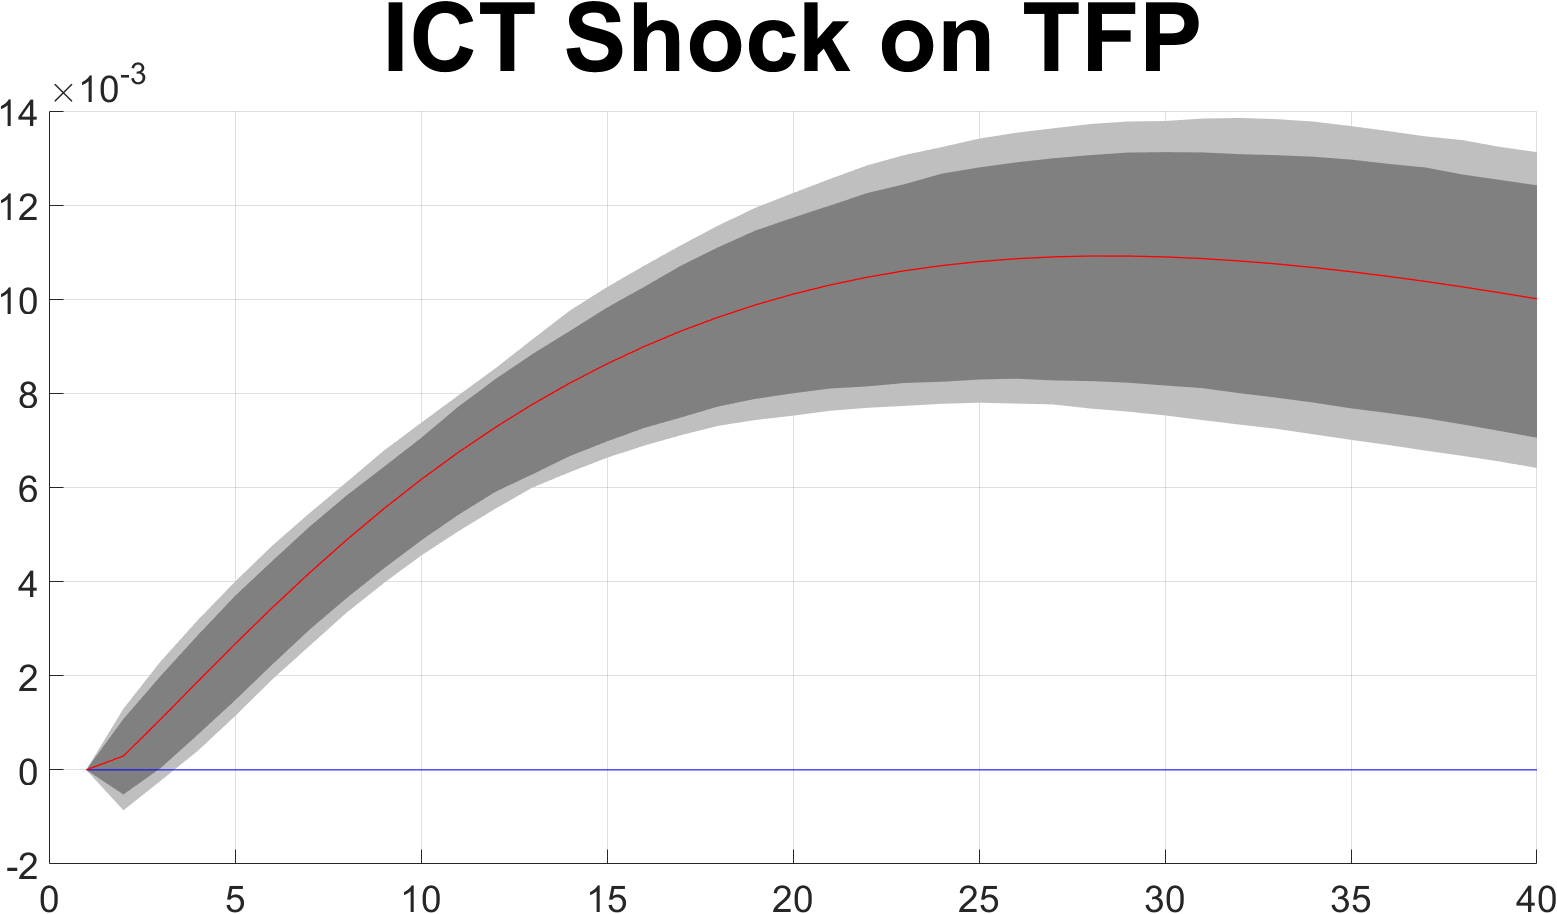
\includegraphics[scale=0.25]{\MainFigures/fig_ICT_Shock_on_TFP_empirical_noH}
\label{fig:TFP_main}
\end{center}
\end{figure}
	

\end{frame}
%%%%%%%%%%%%%%%%%


%%%%%%% Slide %%%%%%
\begin{frame}
	\frametitle{Results II}

\begin{figure}[h!]
%\caption{Best Responses of $\sigma_1^2$} 
%\centering
\subfigure{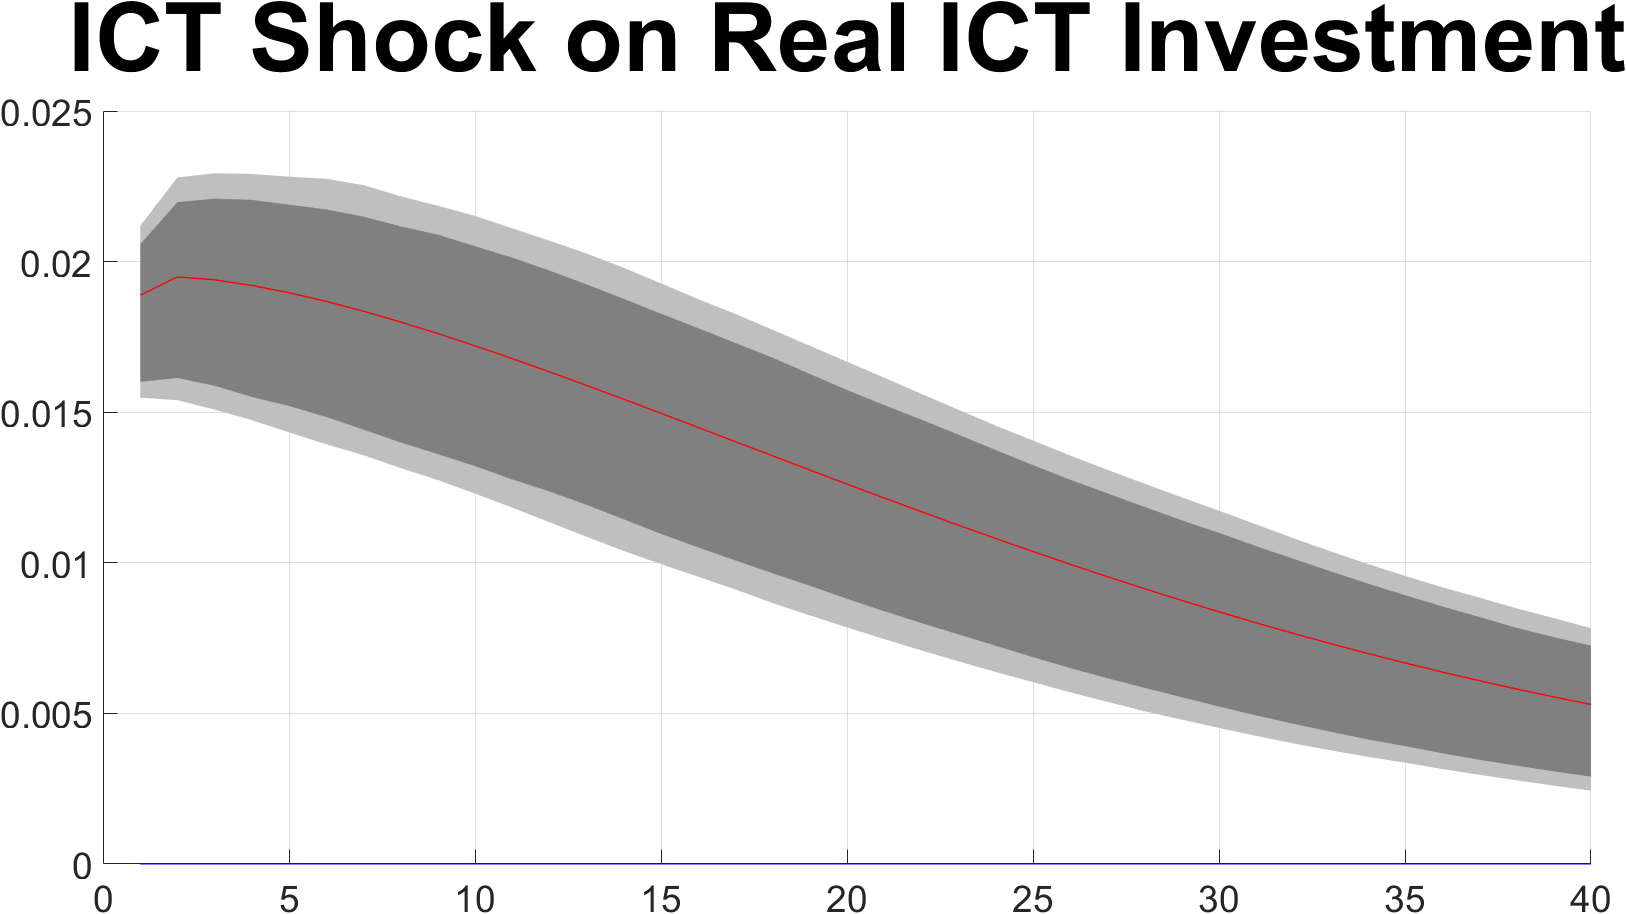
\includegraphics[width=   \myFigWidth]{\MainFigures/fig_ICT_Shock_on_Real_ICT_Investment_empirical_noH}} \hspace{.2in%
} 
\subfigure{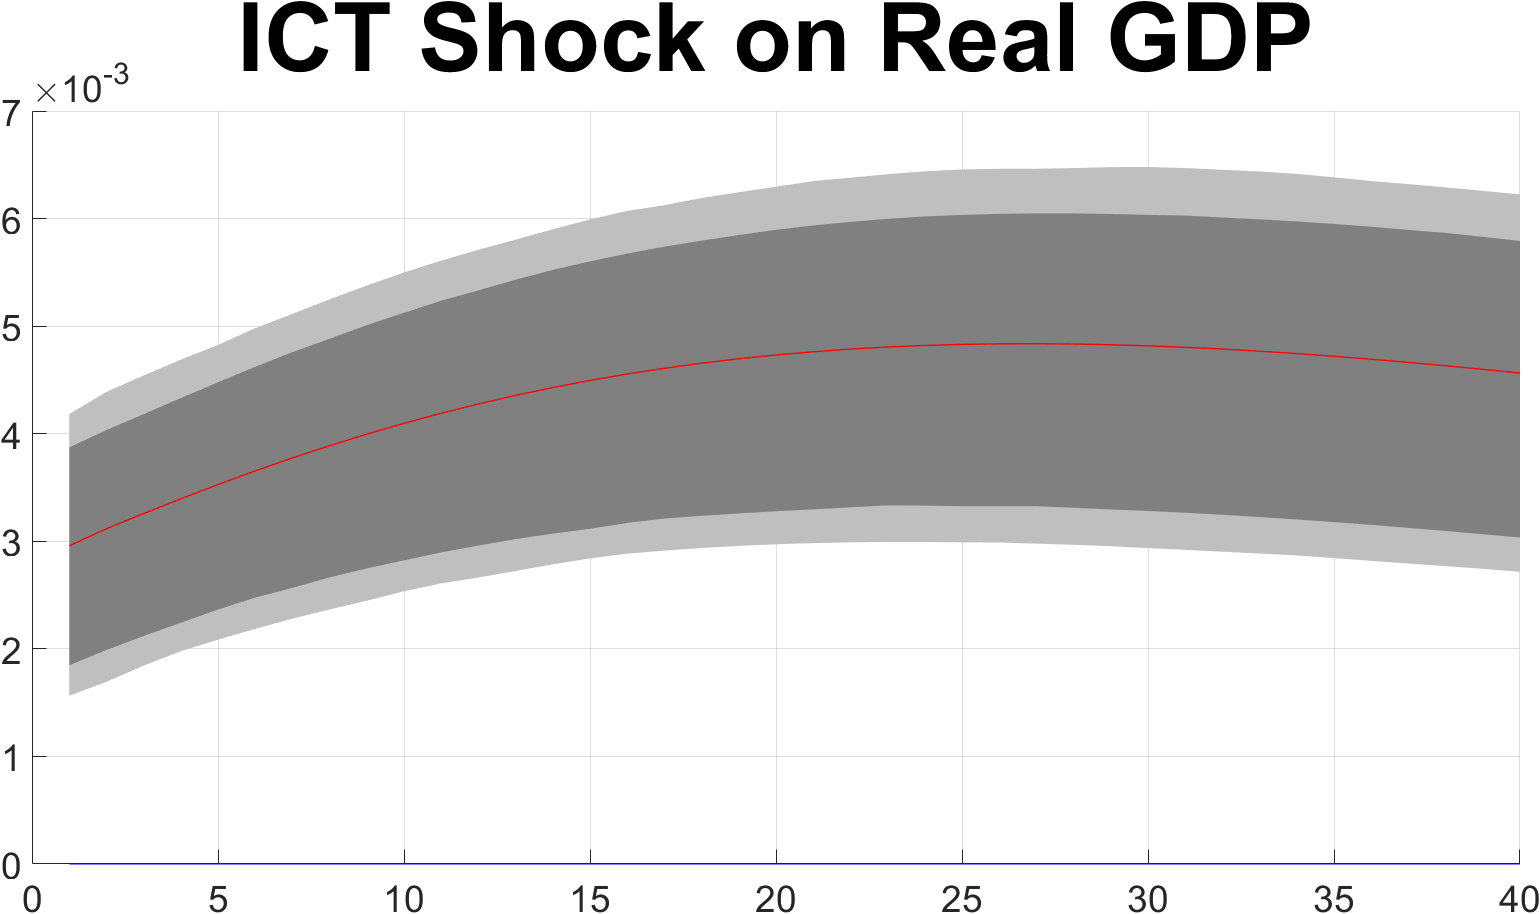
\includegraphics[width=  \myFigWidth]{\MainFigures/fig_ICT_Shock_on_Real_GDP_empirical_noH}} \hspace{.2in%
} 
\subfigure{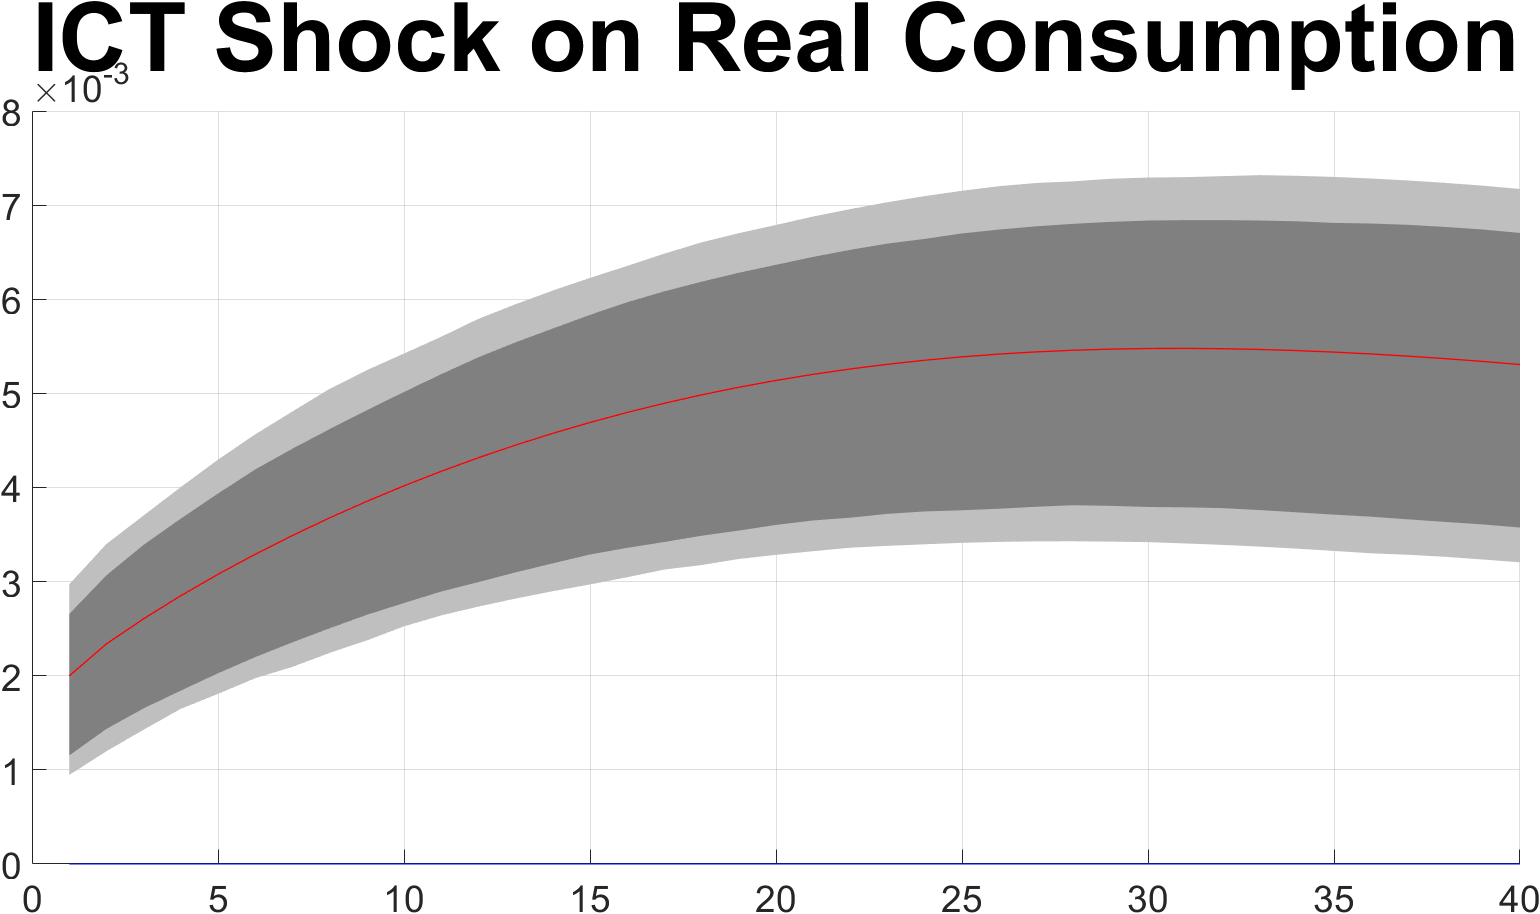
\includegraphics[width=   \myFigWidth]{\MainFigures/fig_ICT_Shock_on_Real_Consumption_empirical_noH}} \hspace{.2in%
} 
\subfigure{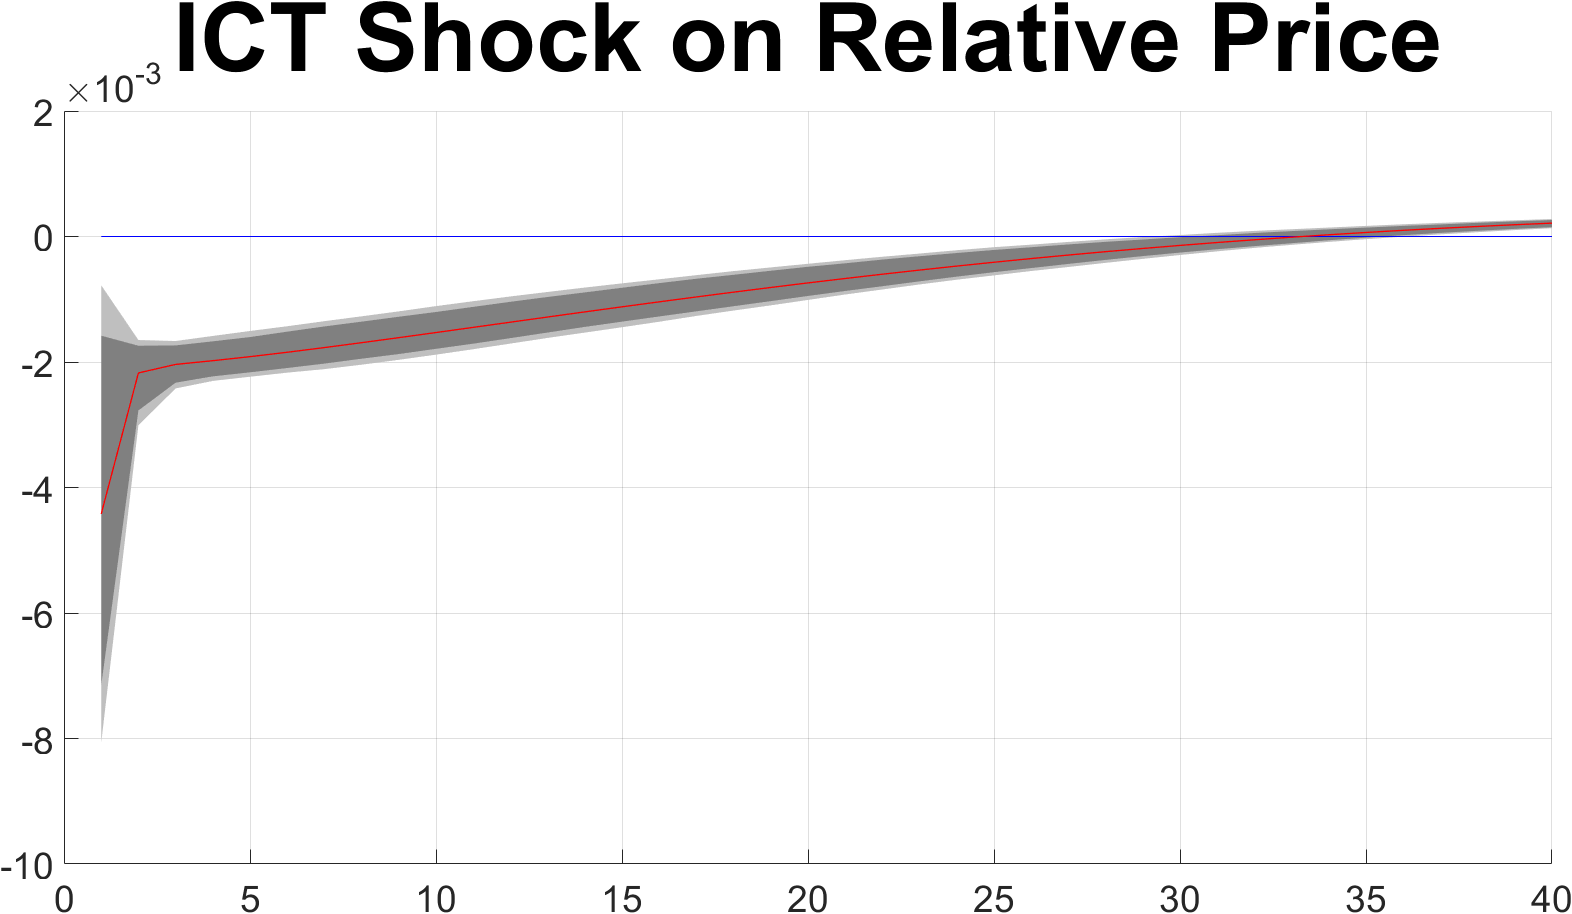
\includegraphics[width=   \myFigWidth]{\MainFigures/fig_ICT_Shock_on_Relative_Price_empirical_noH}} 
\end{figure}	

\end{frame}
%%%%%%%%%%%%%%%%%

%%%%%%% Slide %%%%%%
\begin{frame}
	\frametitle{Results III}
	
\begin{table}[h!]
 		\begin{center}
 \begin{tabular}{lcccccccccc}
\hline
 	& $h = 1$ & $h = 4$ & $h = 8$ & $h = 16$ & $h = 24$ & $h = 40$ \\
 	\hline
TFP &  0       &  0.0023  &  0.0194 &   0.1088 &   0.2273  &  0.3382 \\
ICT-I &  0.9997  &  0.9038  &  0.7964 &   0.6320 &   0.5310  &  0.4371 \\
Real GDP &  0.2620  &  0.3061  &  0.3486 &   0.3936 &   0.4046  &  0.3881 \\
Real C &  0.1952  &  0.2638  &  0.3219 &   0.3931 &   0.4188  &  0.4064 \\
Relative Prices &  0.0618  &  0.0967  &  0.1276 &   0.1511 &   0.1516  &  0.1467 \\	
\hline
 	\end{tabular}
  		%\caption{The letter $h$ denotes the forecast horizon. The numbers refer to the fraction of the forecast error variance of each variable at various forecast horizons to the identified ICT shock}
  \label{table:vardec}
  \end{center}
 \end{table}


\end{frame}
%%%%%%%%%%%%%%%%%

%%%%%%% Slide %%%%%%
\begin{frame}
	\frametitle{Robustness checks}
	\label{robustness_checks}
	
\begin{itemize}
\item Main critique: reverse causality from news about future TFP.

\

\

\item[$\rightarrow$] Alternative specification filters out news to recover an alternative ICT shock series 

\hyperlink{controlling_news}{\beamerbutton{Alternative specification}}	
\end{itemize}

\end{frame}
%%%%%%%%%%%%%%%%%

%%%%%%% Slide %%%%%%
\begin{frame}
	\frametitle{The two recovered ICT shock series}
	
\begin{figure}[h!]
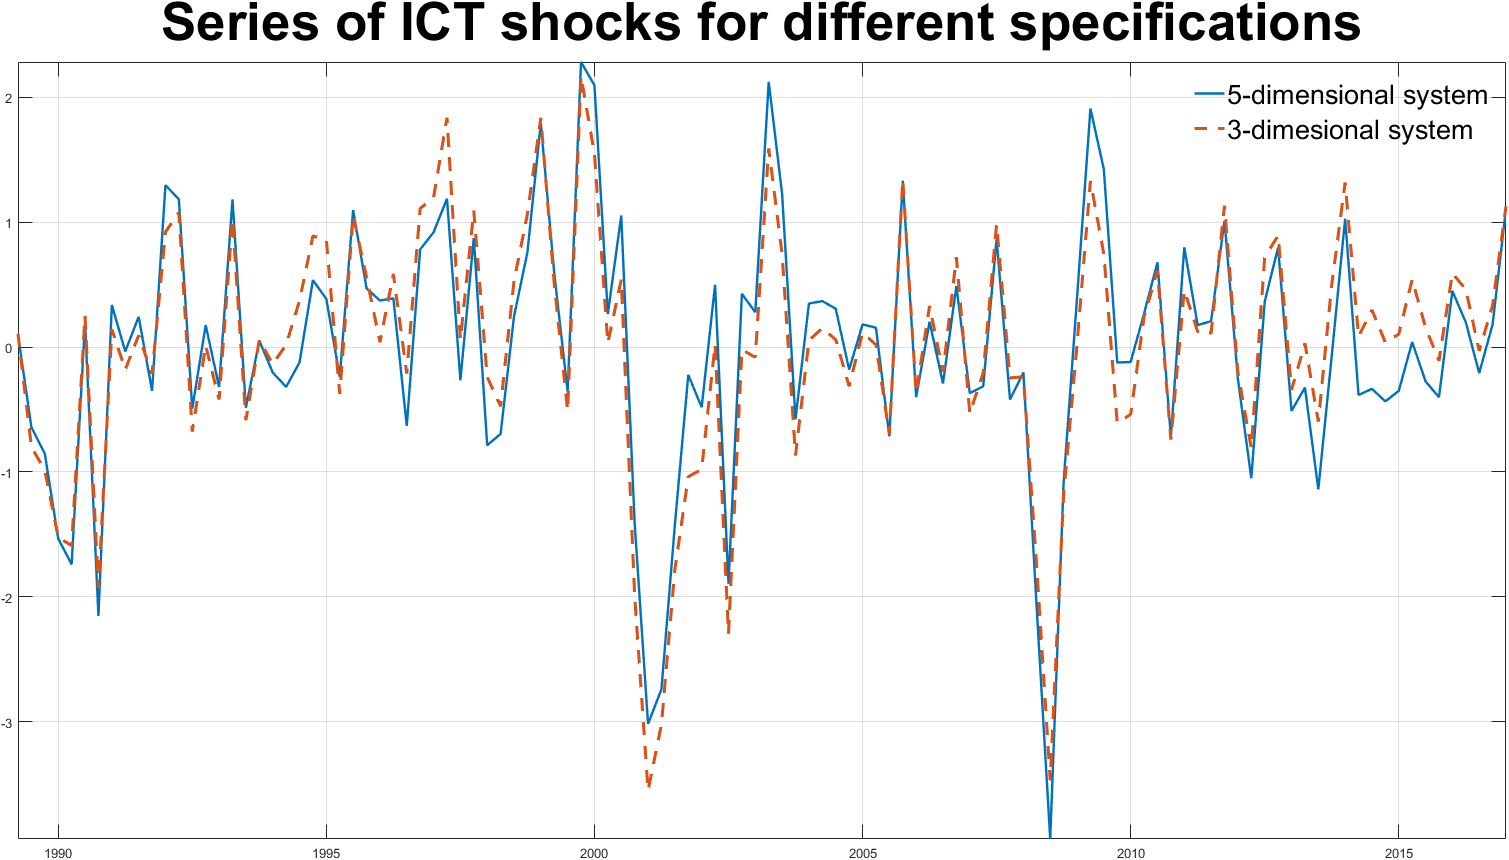
\includegraphics[width=   4.55in]{\MainFigures/Removing_FLVariables}
\end{figure}	

\end{frame}
%%%%%%%%%%%%%%%%%

%%%%%%% Slide %%%%%%
\begin{frame}
	\frametitle{Interpretation of results}
	
	\begin{itemize}
	\item ICT-I leads to significant and persistent TFP increases in the medium run.
	
	\
	
	\
	
	\item ICT literature: it's a general purpose technology (GPT)!
	
	\
	
	\
	
	\item[$\rightarrow$] embed in a structural model and estimate whether data favors the GPT-interpretation.
	\end{itemize}

	
	
	
	

\end{frame}
%%%%%%%%%%%%%%%%%

%%%%%%% Slide %%%%%%
\begin{frame}
\frametitle{Roadmap}

EDIT THIS LATER
\begin{enumerate} 
	\item SVAR analysis: identifying an ICT shock
	
	\
	
	\
	
	\item A two-sector endogenous growth model
	 
	\
	
\end{enumerate} 

\end{frame}
%%%%%%%%%%%%%%%%%

%%%%%%% Slide %%%%%%
\begin{frame}
	\frametitle{2. Model - in a nutshell}
	
	\begin{itemize}
	\item Belongs to the class of (GHK) models 
	
	(we use isomorphic formulation of Oulton)
	
	\
	
	\item Key: two sectors with identical production functions
	\item[$\rightarrow$] with an externality capturing the GPT-nature of ICT-capital.
	
	\
	
	\
	
	\item	Rest of model perfectly standard.
	\end{itemize}
	

\end{frame}
%%%%%%%%%%%%%%%%%

%%%%%%% Slide %%%%%%
\begin{frame}
	\frametitle{Two sectors}

Consumption-good sector
\begin{eqnarray}\label{equation:production_FINAL}
y^c_t(j) = A^c_t \ \big( k^c_{t}(j) \big)^a \ \big( k^i_{t}(j) \big)^b \ \big( l_{t}(j) \big)^{1-a-b}, \ \ 0 < a,b < 1
\end{eqnarray}

\

ICT-good sector
\begin{eqnarray}\label{equation:productionICT}
y^i_t(q) = A_t^i \ \big( k^c_{t}(q) \big)^a \ \big( k^i_{t}(q) \big)^b \ \big( l_{t}(q) \big)^{1-a-b}, \ \ 0 < a,b < 1
\end{eqnarray}

\

with 

\

\centering
$ A_t^c = \eta_t \ \theta^c_t \ \textcolor{red}{(k^i_{t})^{\gamma}}  $

\

$A_t^i = \eta_t \ \theta^i_t \ \textcolor{red}{(k^i_{t})^{\gamma}} $	

\end{frame}
%%%%%%%%%%%%%%%%%

%%%%%%% Slide %%%%%%
\begin{frame}
	\frametitle{Uses of outputs and GDP}

Consumption-good sector

$$
y^c_t = c_t + i^c_t
$$

ICT-good sector


$$
y^i_t = i^i_t
$$

\

GDP is 
$$
GDP_t = (1 - w) y^c_t+ w y^i_t \ \ \ \text{where} \ \ \ w = \frac{p_t y^i_t }{y^c_t + p_t y^i_t }
$$


with

$$
p_t = \frac{p_t^i}{p_t^c} \quad \text{where we normalize} \quad p_t^c = 1
$$



\end{frame}
%%%%%%%%%%%%%%%%%

%%%%%%% Slide %%%%%%
\begin{frame}
	\frametitle{TFP in the model}

Can be computed 2 ways:

\begin{align*}
&1) \;\; TFP_t = (1 - w) TFP_t^c + w TFP_t^i \\
\\
& 2) \;\; g_{TFP} = g_{GDP} - a g_{k^c} -b g_{l} - (1-a-b)g_{k^i}
\end{align*}

\

where for a variable $X$, $g_x \coloneqq \text{ln}\left(\frac{X_t}{X_{t-1}}\right)$.

\

In the model, the latter is equivalent to

\begin{equation}
g_{TFP} = g_{\eta} + wg_{\theta^c} + (1-w)g_{\theta^i} +\textcolor{red}{\gamma}  g_{k^i}
\end{equation}



\end{frame}
%%%%%%%%%%%%%%%%%

%%%%%%% Slide %%%%%%
\begin{frame}
	\frametitle{Impulse-response matching - does data support $\gamma>0$?}
	
Estimate three parameters: $\Omega = (\gamma, \ \sigma_{\iota}^2, \ \rho_{\iota})$ with

\begin{itemize}
\item $\sigma_{\iota}^2 =$ the variance of an ICT technology shock
\item $\rho_{\iota}=$ the persistence of the same shock
\item $\gamma=$  the size of the spillover effect of ICT capital on TFP
\end{itemize}


\

We estimate $\Omega$ as
\begin{eqnarray}\label{equation:min_prob_IRmatching}
\min_{\Omega} \big[  \hat{\Psi} - \Psi(\Omega)  \big]' \Lambda \big[  \hat{\Psi} - \Psi(\Omega)  \big]
\end{eqnarray}

\begin{itemize}
\item $\Psi(\Omega) =$ mapping from $\Omega$ to the theoretical impulse responses
\item $\hat{\Psi} =$ the empirical impulse responses of an ICT shock to TFP, ICTI, C and RP
\end{itemize}

\end{frame}
%%%%%%%%%%%%%%%%%

%%%%%%% Slide %%%%%%
\begin{frame}
	\frametitle{IR-matching results I}

	\begin{table}[h!]
	\begin{center}
		\begin{tabular}{clc}
			\hline
			Symbol & Economic Interpretation & Estimated Value \\
			\hline
            $\sigma^2_{\iota}$ & Variance of ICT technological shock &   $0.01$  \\
            $\rho_{\iota}$     & Persistence of ICT technological shock & $0.9$   \\
            $\gamma$           & Size of spillover of ICT capital on TFP &  $0.5881$ \\
			\hline
		\end{tabular}
		%\caption{Estimation of key parameters by imposing model's impulse responses of an ICT shock to be as close as possible to the empirical ones. Theoretical estimates are impulse responses to an ICT-specific technological shock, $\zeta_t$ which are functions of key parameters: $\sigma_{\iota}^2$, $\rho_{\iota}$, and $\gamma$. Empirical impulse responses of an ICT shock to TFP, ICTI, consumption, and relative prices are derived from Specification \ref{eq:mainSpecification} using the empirical strategy presented in Section \ref{section:empiricalstrategy_simple}. According to what presented in Appendix \ref{section:mainSetResults}, we use a horizon of $40$ periods for each response.}
		\label{table:estimated_parameters}
	\end{center}
\end{table}	

\end{frame}
%%%%%%%%%%%%%%%%%

%%%%%%% Slide %%%%%%
\begin{frame}
	\frametitle{IR-matching results II}
	
\begin{figure}[h!]
%\caption{Best Responses of $\sigma_1^2$} 
%\centering
\subfigure{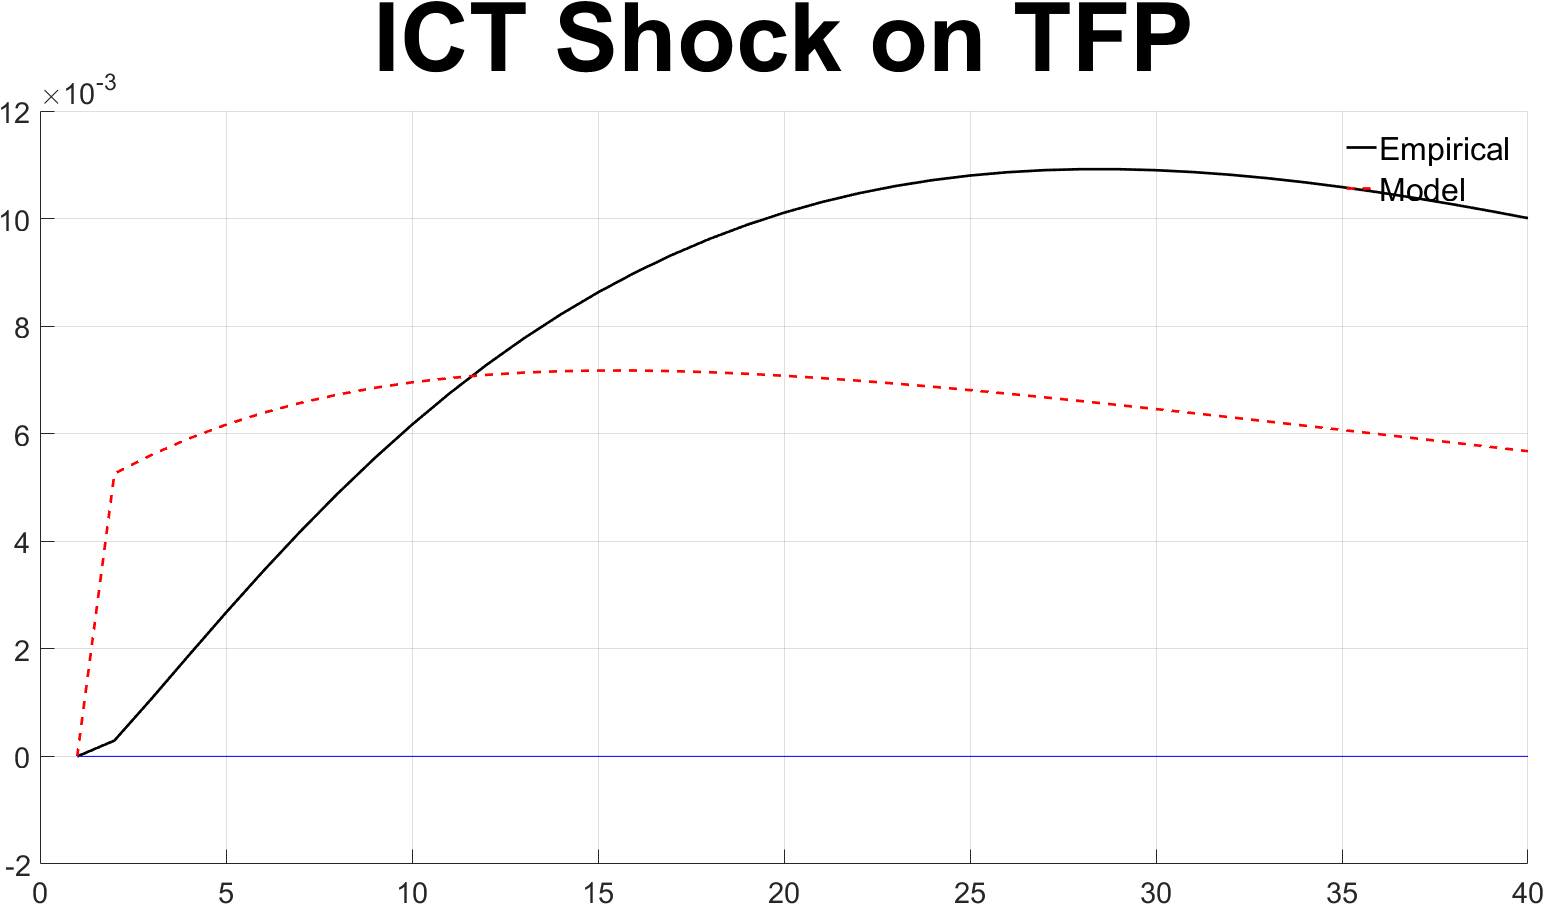
\includegraphics[width=   \myFigWidth]{\MainFigures/fig_ICT_Shock_on_TFP_IRmatching_together}} \hspace{.2in%
} 
\subfigure{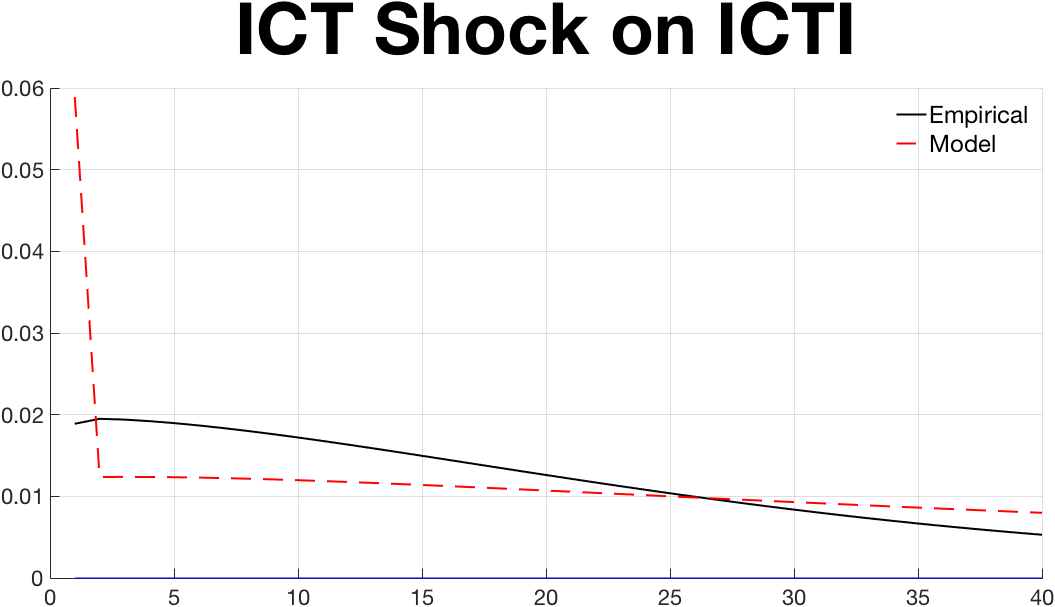
\includegraphics[width=  \myFigWidth]{\MainFigures/fig_ICT_Shock_on_ICTI_IRmatching_together}} \hspace{.2in%
} 
\subfigure{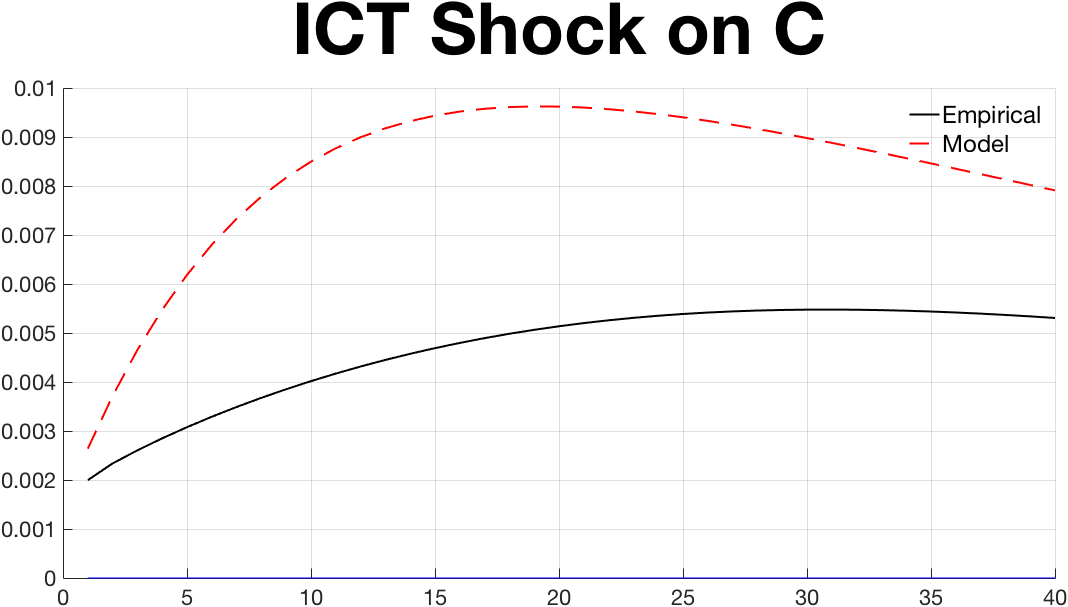
\includegraphics[width=   \myFigWidth]{\MainFigures/fig_ICT_Shock_on_C_IRmatching_together}} \hspace{.2in%
} 
\subfigure{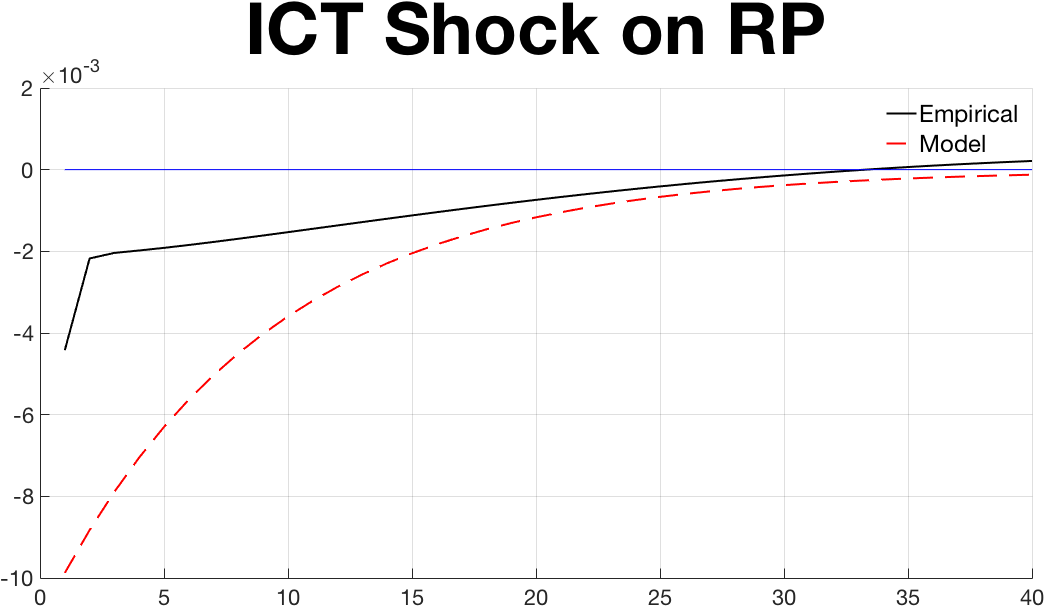
\includegraphics[width=   \myFigWidth]{\MainFigures/fig_ICT_Shock_on_RP_IRmatching_together}} 
\end{figure}
\end{frame}
%%%%%%%%%%%%%%%%%


%%%%%%% Slide %%%%%%
\begin{frame}
	\frametitle{The spillover drives the TFP-response}
\begin{figure}[h!]
\begin{center}
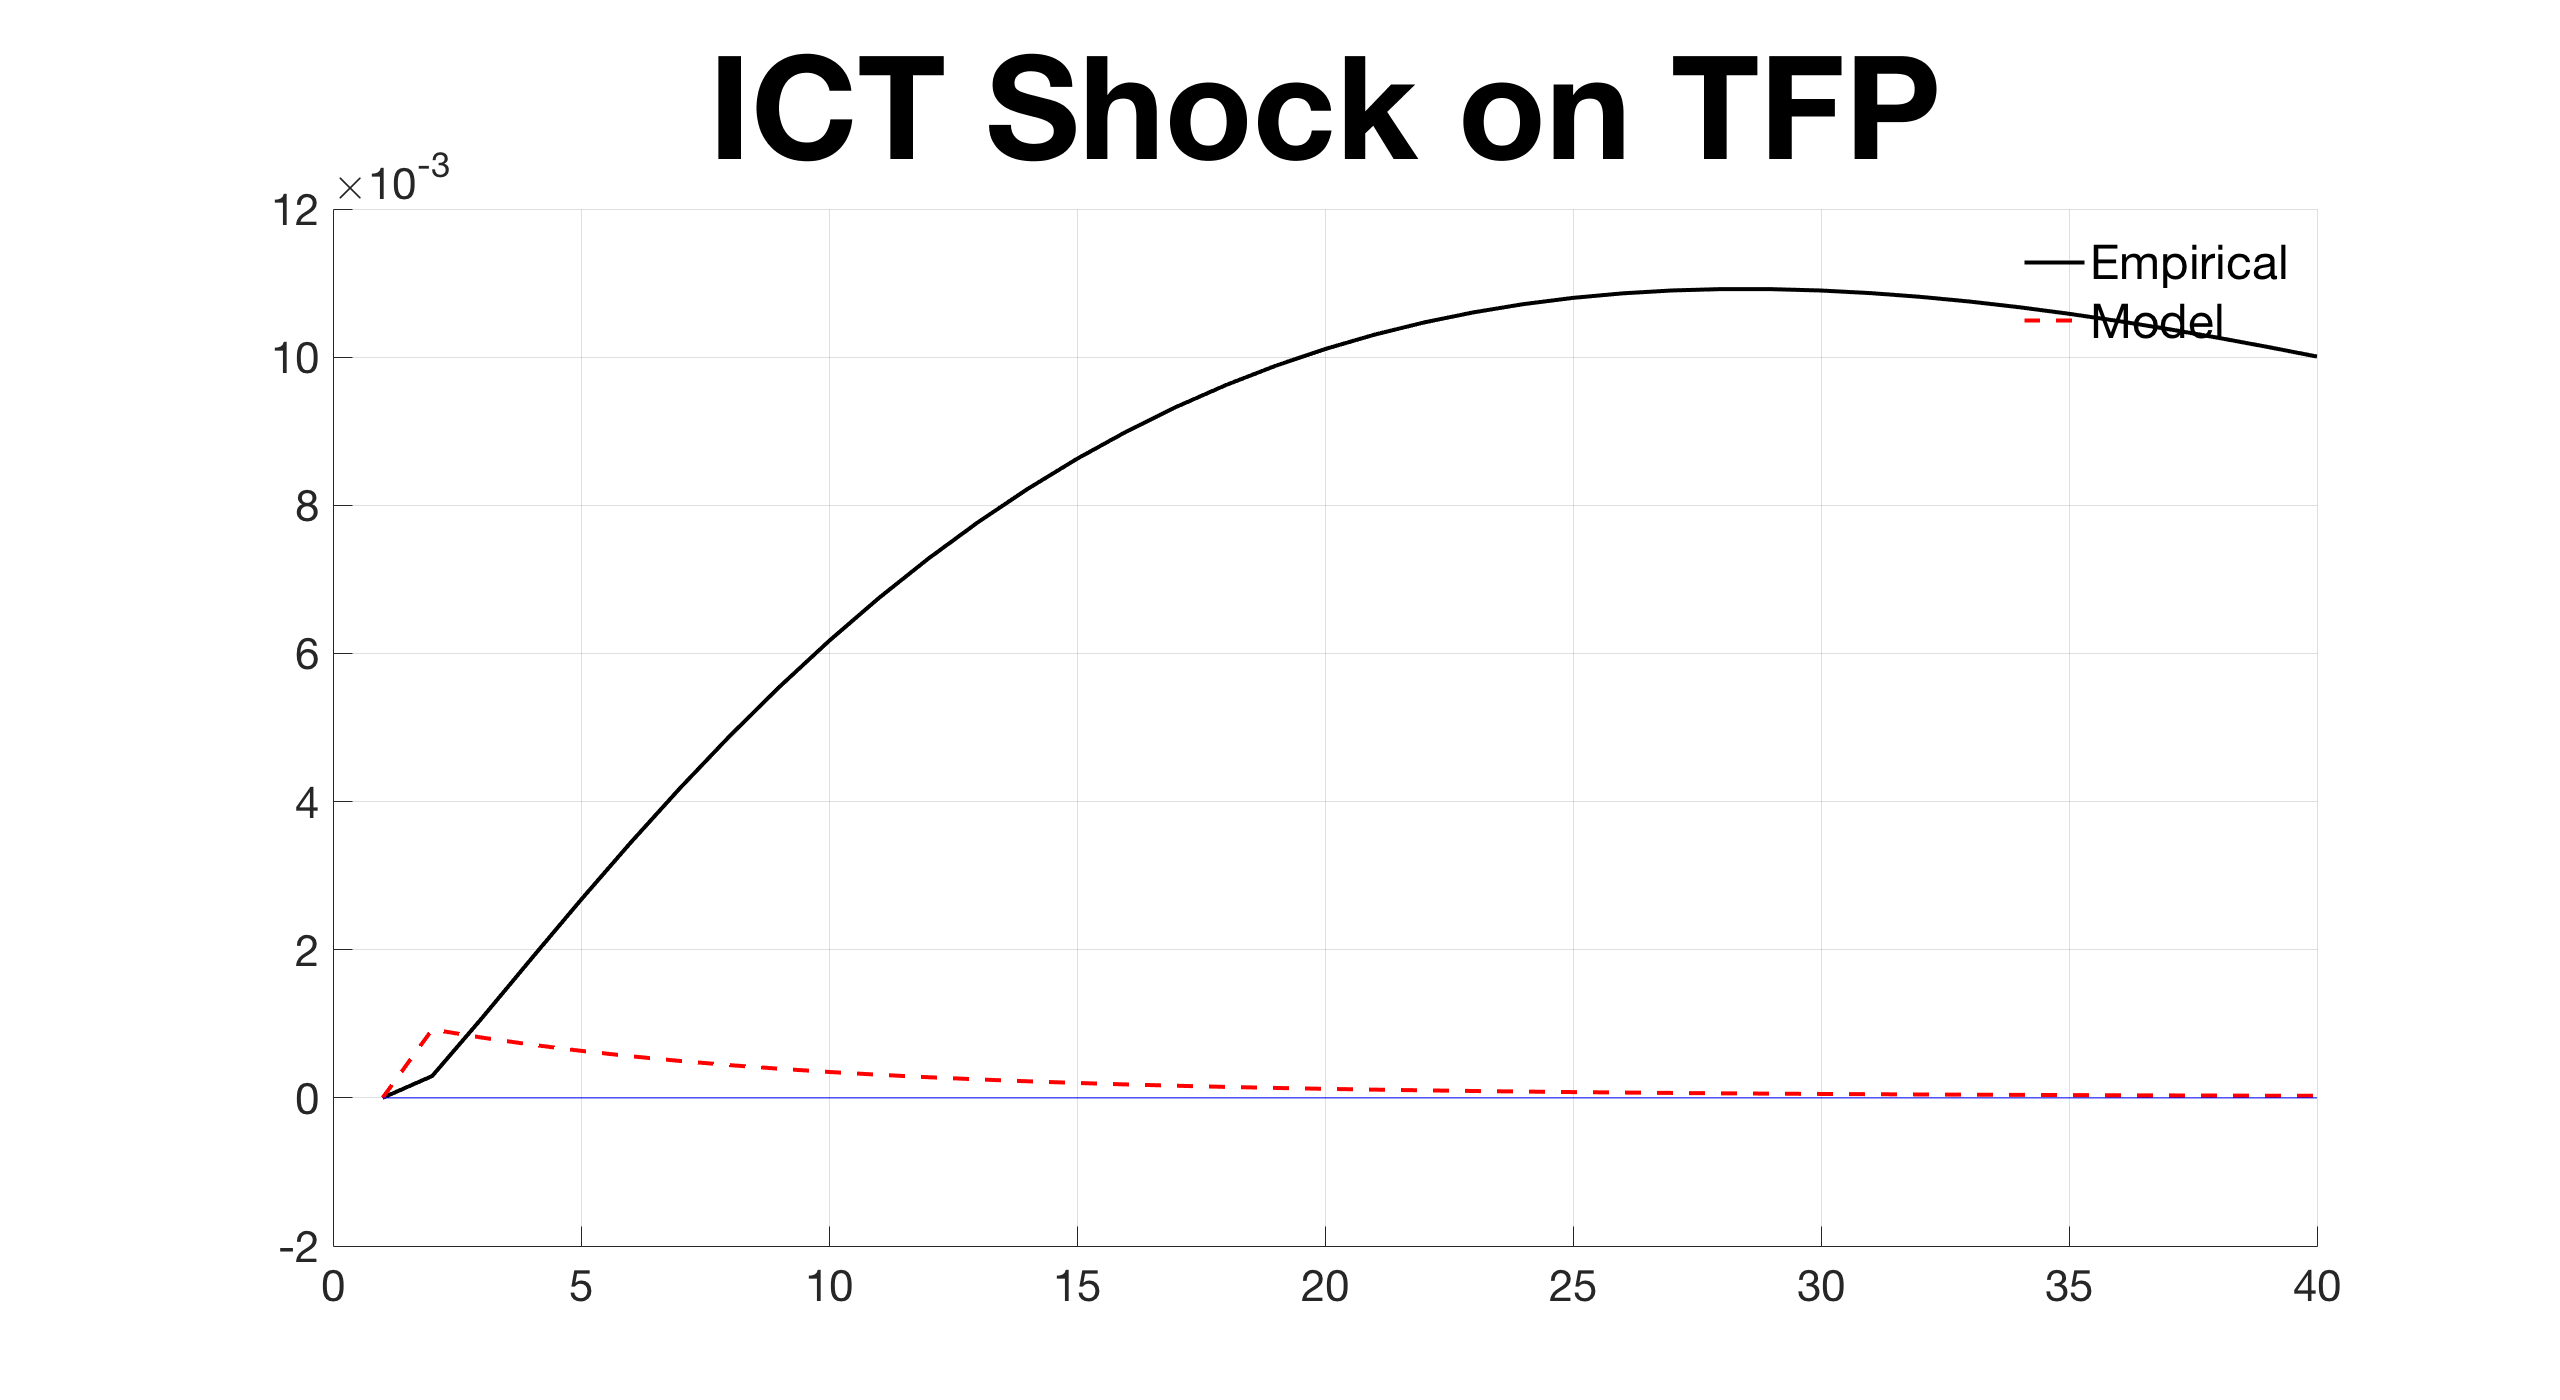
\includegraphics[scale=0.13]{\MainFigures/fig_ICT_Shock_on_TFP_IRmatching_together_gam_set_to0point1}
\caption{Setting $\gamma =0.1$}
\label{fig:TFP_main}
\end{center}
\end{figure}	

\end{frame}
%%%%%%%%%%%%%%%%%


%%%%%%% Slide %%%%%%
\begin{frame}
	\frametitle{Conclusion}

\begin{itemize}
\item SVAR analysis uncovered interesting pattern between ICT productivity and TFP.

\

	\begin{itemize}
	\item[$\rightarrow$] An ICT shock leads to delayed but persistent TFP increases.
	\end{itemize}

\

\

\item Two-sector structural model with a spillover from ICT-capital can rationalize results.

\

	\begin{itemize}
	\item[$\rightarrow$] Estimation of the model suggests that data supports the GPT-interpretation of ICT.
	\end{itemize}
\end{itemize}

	

\end{frame}
%%%%%%%%%%%%%%%%%

%%%%%%% Slide %%%%%%
\begin{frame}
\centering
	THANK YOU!
	

\end{frame}
%%%%%%%%%%%%%%%%%

%%%%%%%%%%%%%%%%%%%%%%%%%%%%%%%%%%%%%%%%%%%%%%%%%%%%%%%%%%%%%%%%%%%%%%
%%%%%%                     APPENDIX  
%%%%%%%%%%%%%%%%%%%%%%%%%%%%%%%%%%%%%%%%%%%%%%%%%%%%%%%%%%%%%%%%%%%%%%


%%%%%%% Slide %%%%%%
\begin{frame}
	\frametitle{Notation in detail}
	\label{VAR_notation}
The reduced-form VAR is
$$
y_t = B(L)y_{t-1} + i_t 
$$

\

Mapping between innovations $i_t$ to structural shocks $s_t$
$$
A_0 s_t = i_t
$$
\

$\rightarrow$ structural-form VAR is
$$
A_0^{-1}y_t = C(L) y_{t-1} + s_t
$$

\

where $C(L) = A_0^{-1} B(L)$ and $s_t = A_0^{-1} i_t$, and the impact matrix $A_0$ satisfies $\Sigma = A_0 A_0'$. 

\end{frame}
%%%%%%%%%%%%%%%%%

%%%%%%% Slide %%%%%%
\begin{frame}
	\frametitle{}

For any arbitrary orthogonalization $\tilde{A}_0 \; : \; \Sigma = \tilde{A}_0 \tilde{A}_0'$, a rotation using an orthogonal matrix $D$ ($DD' = I$) allows us to back out impact matrix as $A_0 = \tilde{A}_0 D$. 

\

$\rightarrow$ The matrix of impact responses to all shocks is: 
$$
\Pi(0) = \tilde{A}_0 D
$$

\

Specifically, denoting the responses of variable $i$ to shock $j$, it is
$$
\Pi_{i,j}(0) = e_i' \tilde{A}_0 D e_j
$$
where $e_k$ is a selector column vector.

Denote $\gamma_j \coloneqq De_j$, a specific column of $D$. 

\

$\rightarrow \tilde{A}_0\gamma_j =$the vector of impact responses of all variables to shock $j$.

\

\hyperlink{baseline_spec}{\beamerreturnbutton{Return}}	
\end{frame}
%%%%%%%%%%%%%%%%%



%%%%%%% Slide %%%%%%
\begin{frame}
	\frametitle{Controlling for news}
	\label{controlling_news}
\textbf{Step 1 - Identification of $\gamma_{news}$} 	

\

\

$$
\max_{\gamma_{news}} \Omega_{1,news}(h) = \frac{ \sum_{t=0}^h e_1' B^t \tilde{A}_0 \gamma_{news} \gamma_{news}' \tilde{A}_0' B'^t e_1 } {e_1' ( \sum_{\tau = 0}^H B^t \Sigma B'^t )e_1}
$$

\

subject to

\

$$
\Pi_{1,news}(0) = 0,
$$
$$
\Pi_{6,news}(0) = \Pi_{6,news}(1) = \Pi_{6,news}(2) = 0, \ \ \text{and}
$$
$$
\gamma_{news} \gamma_{news}' = 1.
$$


\end{frame}
%%%%%%%%%%%%%%%%%

%%%%%%% Slide %%%%%%
\begin{frame}
	\frametitle{Controlling for news}
\textbf{Step 2 - Identification of $\gamma_{ICT}$} 	

\

$$
\max_{\gamma_{ICT}} \Pi_{2,ICT}(0) =  e_2' \tilde{A}_0 \gamma_{ICT} 
$$

\

subject to

\

$$
\Pi_{1,ICT}(0) = 0,
$$
$$
\gamma_{news} \gamma_{ICT}' = 0, \ \ \text{and} \ \ \gamma_{ICT} \gamma_{ICT}' = 1.
$$


\

\
	
\hyperlink{robustness_checks}{\beamerreturnbutton{Return}}	
\end{frame}
%%%%%%%%%%%%%%%%%



%%%%%%% Slide %%%%%%
\begin{frame}
	\frametitle{Robustness checks for the news specification}

\begin{itemize}
\item Different variables
	\begin{itemize}
	\item Add the Michigan index of consumer confidence (expected business conditions 5 years ahead)
	
	
	\
	
	\item Replace IT prices with capital prices (following Comin \& Gertler)
	
	\
	
	\item Replace CPI inflation with PCE inflation
	\end{itemize}
	
	\
	
\item Different horizons at which we impose the restriction on relative prices for the news shock
\item[] $\rightarrow$ ran  6, 8, 10, 12 and 16 quarters.

\

\item Increase the number of lags (2)

\

\item Check whether VAR is information-sufficient to identify the news shock (Forni-Gambetti test) (p-val of 12\%)
\end{itemize}

\

\hyperlink{robustness_checks}{\beamerreturnbutton{Return}}	

   		 	
\end{frame}
%%%%%%%%%%%%%%%%%




\end{document}
